%Standard stuff
\documentclass[a4paper,10pt,english]{article}
\usepackage[utf8]{inputenc}
\usepackage[english]{babel}
\usepackage{amsmath,graphicx,varioref,verbatim,amsfonts,geometry,enumerate,commath,textcomp,listings,siunitx,float}
% colors in text
\usepackage[usenames,dvipsnames,svgnames,table]{xcolor}
% Hyper refs
\usepackage[colorlinks]{hyperref}
% inkspace
\usepackage{import}
\usepackage{xifthen}
\usepackage{pdfpages}
\usepackage{transparent}
\usepackage{tikz,pgfplots,cancel}

%Biber
\usepackage[backend=biber, style=chicago-authordate]{biblatex}
\AtEveryBibitem{%
	\clearlist{language}}

% Colour scheme for hyperlinks
\hypersetup{%
	colorlinks,
	citecolor=Blue,
	linkcolor=Blue,
	urlcolor=Blue}

% Document formatting
\setlength{\parindent}{0mm}
\setlength{\parskip}{1.5mm}
\definecolor{mygreen}{RGB}{28,172,0} % color values Red, Green, Blue
\definecolor{mylilas}{RGB}{170,55,241}
% Color scheme for listings
\usepackage{textcomp}
\definecolor{codegreen}{rgb}{0,0.6,0}
\definecolor{codegray}{rgb}{0.5,0.5,0.5}
\definecolor{codepurple}{rgb}{0.58,0,0.82}
\definecolor{backcolour}{rgb}{0.95,0.95,0.92}
\definecolor{listinggray}{gray}{0.9}
\definecolor{lbcolor}{rgb}{0.9,0.9,0.9}
\lstdefinestyle{mystyle}{
	backgroundcolor=\color{backcolour},
	commentstyle=\color{codegreen},
	keywordstyle=\color{magenta},
	numberstyle=\tiny\color{codegray},
	stringstyle=\color{codepurple},
	basicstyle=\ttfamily\footnotesize,
	breakatwhitespace=false,
	breaklines=true,
	captionpos=b,
	keepspaces=true,
	numbers=left,
	numbersep=5pt,
	showspaces=false,
	showstringspaces=false,
	showtabs=false,
	tabsize=2
}

\lstset{style=mystyle}

%for toc
\usepackage{tocloft}
\addtolength{\cftsubsecnumwidth}{40pt}

% new commands
\newcommand{\dd}[1]{\mathrm{d}#1}
\def\doubleunderline#1{\underline{\underline{#1}}}
\newcommand{\uvec}[1]{\boldsymbol{\hat{\textbf{#1}}}}
\renewcommand{\thesection}{Problem \arabic{section}}
\renewcommand{\thesubsection}{\thesection.\alph{subsection})}

%ne pas modifier ou enlever la ligne ci-haut
% \documentclass[11pt,letterpaper]{article}

%2015-08-26 - Document préparé par David Lafrenière, pour le cours PHY1234.

%Pour langue et caractères spéciaux
% \usepackage[english]{babel}
% \usepackage[T1]{fontenc}
% \usepackage{lmodern}
% \usepackage[utf8]{inputenc}
% \usepackage{multicol}
% \usepackage{gensymb}
% \usepackage{MnSymbol}
% \usepackage{xcolor}
% \usepackage{soul}
% \usepackage{units}
% \usepackage{makecell}
% \usepackage{wasysym}
% \usepackage{subfig}
% \usepackage{listings}
% \usepackage{amsmath}
% \usepackage{physics}
% \usepackage[usenames,dvipsnames,svgnames,table]{xcolor}
% \usepackage[colorlinks]{hyperref}

% \definecolor{codegreen}{rgb}{0,0.6,0}
% \definecolor{codegray}{rgb}{0.5,0.5,0.5}
% \definecolor{codepurple}{rgb}{0.58,0,0.82}
% \definecolor{backcolour}{rgb}{0.95,0.95,0.92}

% %Biber
% \usepackage[backend=biber, style=chicago-authordate]{biblatex}
%   \AtEveryBibitem{%
	%     \clearlist{language}}

% % Colour scheme for hyperlinks
%   \hypersetup{%
	%     colorlinks,
	%     citecolor=Blue,
	%     linkcolor=Blue,
	%     urlcolor=Blue}

% \lstdefinestyle{mystyle}{
	%     backgroundcolor=\color{backcolour},
	%     commentstyle=\color{codegreen},
	%     keywordstyle=\color{magenta},
	%     numberstyle=\tiny\color{codegray},
	%     stringstyle=\color{codepurple},
	%     basicstyle=\ttfamily\footnotesize,
	%     breakatwhitespace=false,
	%     breaklines=true,
	%     captionpos=b,
	%     keepspaces=true,
	%     numbers=left,
	%     numbersep=3pt,
	%     showspaces=false,
	%     showstringspaces=false,
	%     showtabs=false,
	%     tabsize=2
	% }

% \lstset{style=mystyle}


% %Pour ajuster les marges
% %\usepackage[top=2cm, bottom=2cm, left=1.4cm, right=1.4cm, columnsep=20pt]{geometry}


% %pour inclure des graphiques
% \usepackage{graphicx}
% \usepackage{float}
% \usepackage{amsmath}

% %Pour inclure des adresse web
% \usepackage{url}

% %pour inclure les codes en annexe
% \usepackage{fancyvrb}
% \usepackage{listingsutf8}
% \usepackage{color}
% \lstset{inputencoding=utf8/latin1,numbers=left,numberstyle=\footnotesize,frame=single,commentstyle=\it\color{blue},keywordstyle=\bf\color{red}}
\addbibresource{../../../refs/refs.org} % Entries are in the "refs.bib" file

\begin{document}
	
	%Page titre
	% \begin{titlepage}
		% \center
		
		% \vspace*{2cm}
		
		% \textsc{\LARGE University of Oslo}\\[1cm]
		% \textsc{\Large FYS4150-3150}\\[1.5cm]
		
		% \rule{\linewidth}{0.5mm} \\[0.5cm]
		% {\LARGE \bfseries Project 1} \\[0.2cm] % ***éditez ceci***
		% \rule{\linewidth}{0.5mm} \\[5cm]
		
		% \textbf{\Large  Martaillé Richard Eloi}\\
		% %{\Large Student number : 669517}\\[8cm]
		% \textbf{\Large  Vebjørn Øvereng}\\
		% \textbf{\Large  Christophe Kristian Blomsen}\\
		% \textbf{\Large  Vetle Henrik Hvoslef}\\
		% % this was not very pretty
		
		\author{Christophe Kristian Blomsen\\
			\texttt{c.k.blomsen@astro.uio.no}
			\and
			Eloi Martaillé Richard\\
			\texttt{e.m.richard@astro.uio.no}
			\and
			Vebjørn Øvereng\\
			\texttt{vebjoro@uio.no}
			\and
			Vetle Henrik Hvoslef\\
			\texttt{vetlehh@uio.no}}
		\title{Project 2}

			\begin{titlepage}
				\maketitle
				\tableofcontents
				
			\end{titlepage}
			
			%\include{sections/method}
			
			Github page: \url{https://github.com/christopheblomsen/project2}
			
			\section{} % problem 1
				Will start from the definitions
				\begin{align}
				  \gamma \frac{\dd{u^{2}}}{\dd{x^{2}}} &= -Fu\\
				  \frac{\dd{u^{2}}}{\dd{x^{2}}}&= - \frac{F}{L}u \label{eq:2}
				\end{align}
				Now using
				\begin{align}
				  \hat{x} &= \frac{x}{L}\\
						  &\Downarrow\nonumber\\
				  \frac{\dd{}}{\dd{x}} &= \frac{\dd{}}{\dd{\hat{x}}}\frac{\dd{\hat{x}}}{\dd{x}}\\
						  \frac{\dd{}}{\dd{x}} &= \frac{\dd{}}{\dd{\hat{x}}} \frac{1}{L}\\
				  &\Downarrow\nonumber\\
				  \frac{\dd{^{2}}}{\dd{x^{2}}} &= \frac{\dd{^{2}}}{\dd{\hat{x}^{2}}}\frac{1}{L^{2}}\label{eq:1}
				\end{align}
				Putting \eqref{eq:1} into \eqref{eq:2}
				\begin{align}
				  \frac{1}{L^{2}}\frac{\dd{^{2}u}}{\dd{\hat{x}^{2}}} &= - \frac{F}{\gamma}u\\
				  \frac{\dd{^{2}u}}{\dd{\hat{x}^{2}}} &= -\frac{FL^{2}}{\gamma} u\\
				  \frac{\dd{^{2}u}}{\dd{\hat{x}^{2}}} &= -\lambda u
				\end{align}
				
We use the fact that since we both scale $u_x(x)$ and
$x$ so that they become $u_{\hat{x}}(\hat{x})$ and $\hat{x}$, we can say that $u_x(x) = u_{\hat{x}}
(\hat{x})$. Because we have both scaled the function
and its interval so $u_x(x)$ on the interval $x \in
[0, L]$ and $u_{\hat{x}}(\hat{x})$ on $\hat{x} \in
[0, 1]$ should look the same. Using this we have that 

\begin{align}
	\frac{\dd{^{2}u}}{\dd{\hat{x}^{2}}} &= -\lambda u \\
	\frac{\dd{^{2} u_{\hat{x}}(\hat{x})}}{\dd{\hat{x}^{2}}} 
	&= - \lambda u_{\hat{x}}(\hat{x})
\end{align}

			\section{} % problem 2
			In order to solve our system, we have to set up a tridiagonal matrix $\boldmath{A}$
			so we have implemented a function in our \lstinline{src/utils.cpp}
called \lstinline{create_tridiagonal}.  This function takes 3 double numbers a,
d, e representing the number on each line. We first initialize our matrix with
setting it up as our identity matrix multiplied by our diagonal number d. Next
we iterate over every row until the last one, where for each row i we assigned
the two values
			$a_{i, i+1} = e$ and $a_{i+1, i} = a$ creating our tridiagonal matrix $\boldsymbol{A}$.\\
			
			To test if our matrix is correctly set up and can correspond to our system, we have 
			calculated the analytical eigenvalues and eigenvectors given in the
Project description and we used the armadillo \lstinline{arma::eig_sym} on our
matrix to compare with the analytical solution. We did obtain the same results
with both methods showing that our matrix was successfully set up. We can find
the test while running the \lstinline{main.cpp} file.
			
			\section{} % problem 3
			\subsection{}
			One main point in the Jacobi's rotation method is to find the maximum off-diagonal element of our matrix. So we created a \lstinline{max_offdiag_symmetric} to find our maximum off-diagonal element assuming a symmetric matrix allowing us to only iterate over the upper part of our matrix considerably reducing the computational time. \\
			
			We start off by defining the row size our matrix and initializing our maximum value b to be 0 so we are sure to replace in our first iteration since we consider the absolute value. Then we create a double for loop, the first one iterates on every row and the other will iterate on every upper element of that row, i.e, for a row i we will iterate over every $j>i$ and compare that element to our current maximum absolute value.  
			
			
			\subsection{}
			We have implemented the function in \lstinline{src/utils.cpp} and to do the test with the required matrix we can run the \lstinline{test_3.cpp} file.
			
			
			\section{} % problem 4
			\subsection{}
			A single Jacobi rotation is performed by
			\lstinline{jacobi_rotate()}. First we calculate $\tau$ as

			\begin{equation}
			\tau = \frac{a_{\text{ll}}^{\text{m}}
			 - a_{\text{kk}}^{\text{m}}}{2a_{\text{kl}}^{\text{m}}},
			\end{equation}

			then we find $\tan \theta$, $\sin \theta$
			and	$\cos \theta$. We choose the
			smallest of the two possible angles of
			rotation, that is
			\begin{equation}
			  \tau = \begin{cases}
				\tan \theta = \frac{1}{\tau + sqrt{1 +
					\tau^2}}, &\quad \tau \geq 0\\
				\tan \theta = \frac{-1}{-\tau + \sqrt{1 +
					\tau^2}}, &\quad \tau < 0. \\
			  \end{cases}
			  \end{equation}
			$\sin \theta$ and $\cos \theta$ are
			calculated found by
			\begin{align}
			  \cos \theta =& \frac{1}{\sqrt{1 + \tan^2\theta}}\\
			  \sin \theta =& \cos \theta \tan \theta.\\
			  \end{align}


			We can now perform the rotation on the  $\bold{A}$-matrix, $\bold{A}^{\text{m}} \rightarrow \bold{A}^{\text{m+1}}$,   first we update the four elements $a_{\text{kk}}$, $a_{\text{ll}}$, $a_{\text{kl}}$ and $a_{\text{lk}}$
			\begin{align}
			  a_{\text{kk}}^{\text{m+1}} =& a_{\text{kk}}^{m}\cos^2\theta - 2 a_{\text{kl}}^{m} \cos \theta \sin \theta + a_{\text{ll}}^{m} \sin^2\theta \\
              a_{\text{ll}}^{m+1} =& a_{\text{ll}}^{m}\cos^2 \theta + 2a_{\text{kl}}^{m}\cos \theta \sin \theta + a_{\text{kk}}^{m}\sin \theta \\
              a_{\text{kl}}^{m+1} =& a_{\text{lk}}^{m+1} = 0,  \\
\end{align}
            and then the rows and columns given by ${k, l}$. For all $i \neq k, l$
\begin{align}
            a_{\text{ik}}^{m+1} =& a_{\text{ik}}^{m}\cos \theta - a_{\text{il}}^{m} \\
            a_{\text{ki}}^{m+1} =& a_{\text{ik}}^{m+1} \\
            a_{\text{il}}^{m+1} =& a_{\text{il}}^{m}\cos \theta + a_{\text{ik}}^{m} \sin\theta \\
            a_{\text{li}}^{m+1} =& a_{\text{il}}^{m+1}.
\end{align}

We make sure to store $a_{\text{kk}}^{m}$ and $a_{\text{ik}}^{m}$ not to unintentionally use the next step
$m+1$ in the updates.

Now we update our rotation matrix $\bold{R}^{\text{m}} \rightarrow \bold{R}^{\text{m+1}} = \bold{R}^{\text{m}}\bold{S}_{\text{m}}$. For all $i$
\begin{align}
r_{\text{ik}}^{m+1} =& r_{\text{ik}}^{m}\cos\theta - r_{\text{il}}^{m}\sin\theta \\
r_{\text{il}}^{m+1} =& r_{\text{il}}^{m}\cos\theta - r_{\text{ik}}^{m}\sin\theta \\
\end{align}

For å implementere heile løysingsalgoritmen lager me funksjonen \lstinline{jacobi_eigensolver()},
denne kallar på \lstinline{max_offdiag_symmetric()} for å finne indeksane \lstinline{k} og \lstinline{l} og
utførar Jacobi-rotasjonar iterativt for å iterere vekk desse elementa fram til det største elementet er
mindre enn ein toleranse.


			\subsection{}
            We implement the analytical solution in the functions \lstinline{analytical_eigenvalues()} and
            \lstinline{analytical_eigenvectors()}. We solve for the eigenvectors of the $6\times 6$-matrix
            given in the project description.

			\begin{figure}[ht]
			  \centering
			  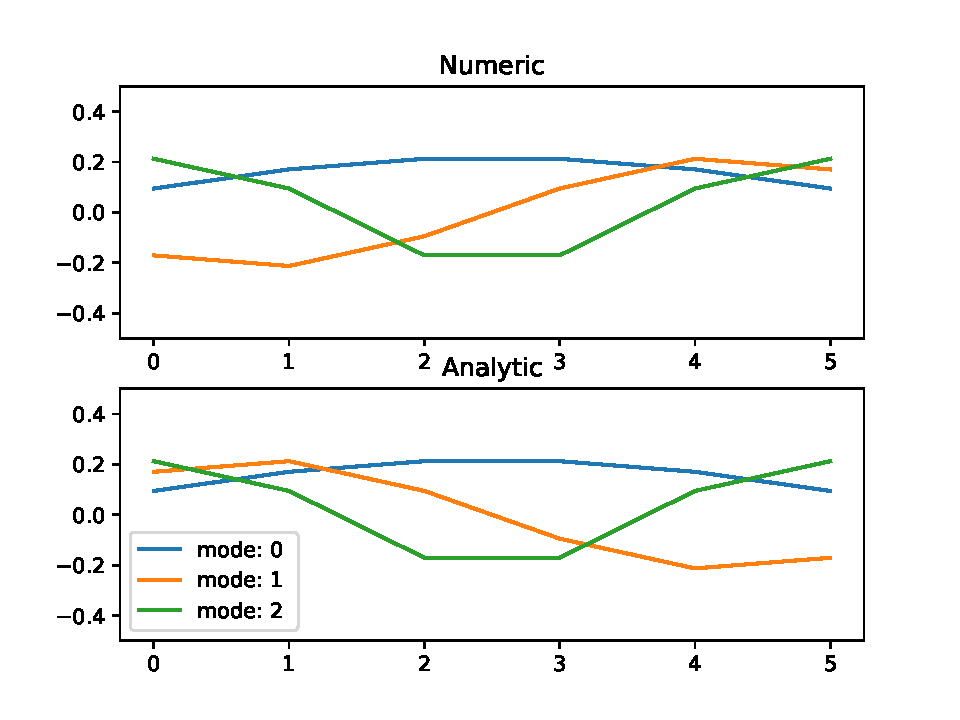
\includegraphics[width=1.0\linewidth]{figures/problem4b.pdf}
			  \caption{The first three eigenvectors of our 6x6 test matrix. With the exception that mode 2 is flipped they look similar.}
              \label{fig:prob4b}
			\end{figure}


            In \autoref{fig:prob4b} we can see two plots comparing the first three eigenvectors. By eye they
            seem similar. If we divide the analytical solution by the numerical solution element wise we get a
            constant vector of ones. This is conclusive that the solutions are indeed identical, our
            implementation of Jacobi's rotation method is up and running.

			
			\section{} % problem 5
			\subsection{}

			This is achieved with a for loop running over $N$ from 10 to 100 with the iteration being multiplied by a factor $10$ for each of them
			\begin{figure}[ht]
			  \centering
			  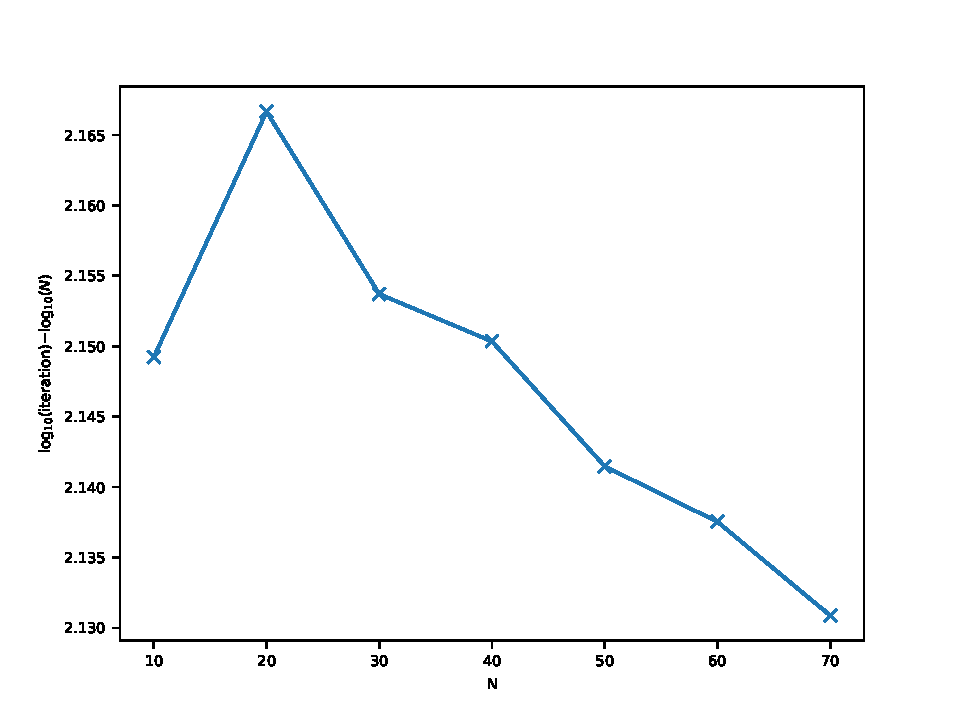
\includegraphics[width=1.0\linewidth]{figures/prob5.pdf}
			  \caption{A logarithmic y axis showing the level of $N$ needed to get to convergence with the Jacobi method\label{fig:prob5}}

			\end{figure}
			See in  \autoref{fig:prob5} that we need roughly $N^{2.13}$ iterations for the algorithm to converge,
			and that this number is fairly constant over the range we tested.

			This can also be seen in the table
			\begin{table}
			  \centering
			  \caption{Table of the different $N$ with corresponding iterations and the log difference. \label{tab:prob5}}
			  \begin{tabular}{||c|c|c||}
				\hline
				$N$              &Iterations    &$\log_{10}$(Iter)-$\log_{10}$(N)               \\
				\hline
				\hline
                      10                     &141                 &2.14922                       \\
				\hline
                      20                     &659                 &2.16666                       \\
				\hline
                      30                    &1518                  &2.1537                       \\
				\hline
                      40                    &2786                 &2.15034                       \\
				\hline
                      50                    &4348                 &2.14147                       \\
				\hline
                      60                    &6322                 &2.13753                       \\
				\hline
                      70                    &8544                 &2.13087                       \\
				\hline
			  \end{tabular}
			  \end{table}
			  Reason why $N>70$ is not included in both \autoref{fig:prob5} and \autoref{tab:prob5} is that it did not converge.


			\subsection{}

We will except the same behavior in the algorithm with a dense

matrix as with a matrix with lots zeros. In the \lstinline{max_offdiag_symmetric()}
we check all the values of the upper triangle regardless of zero or
not, so that would stay the same. That is also because we assume that
the dense matrix is still an symmetric matrix, so we still only need
to care about, in our case, the upper triangle.


The reason for the Jacobi rotation algorithm to approximately take the
same time is because of the fact that when we rotate one max value to
be zero other values that previously were zero may then become not
zero. \cite{morten:compphys}


			\section{} % problem 6
			\subsection{}
			The figure can be seen in~\autoref{fig:6a}
            \begin{figure}[ht]
              \centering
              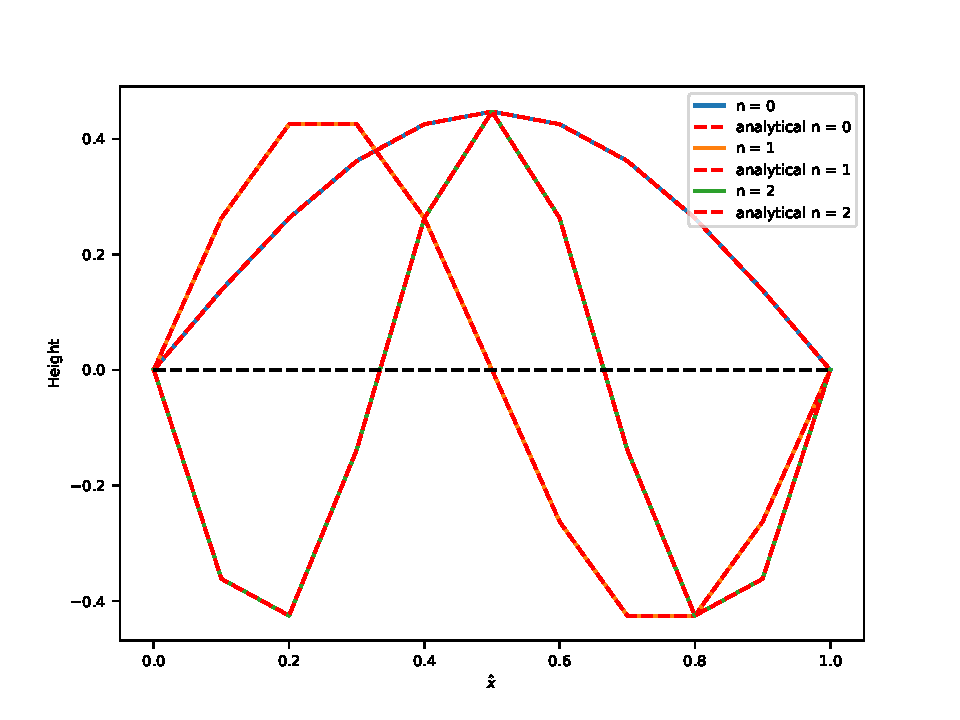
\includegraphics[width=1.0\linewidth]{figures/prob_6a.pdf}
              \caption{Numerical solution for the first three mode in plain line with the analytical solution for the same mode in red dashed line for N=10. The solution is presented with the dimensionless scale $\hat{x}$ is on the $x$-axis, and the amplitude is on the $y$-axis\label{fig:6a} }
            \end{figure}

			\subsection{}

			\begin{figure}[ht]
				\centering
				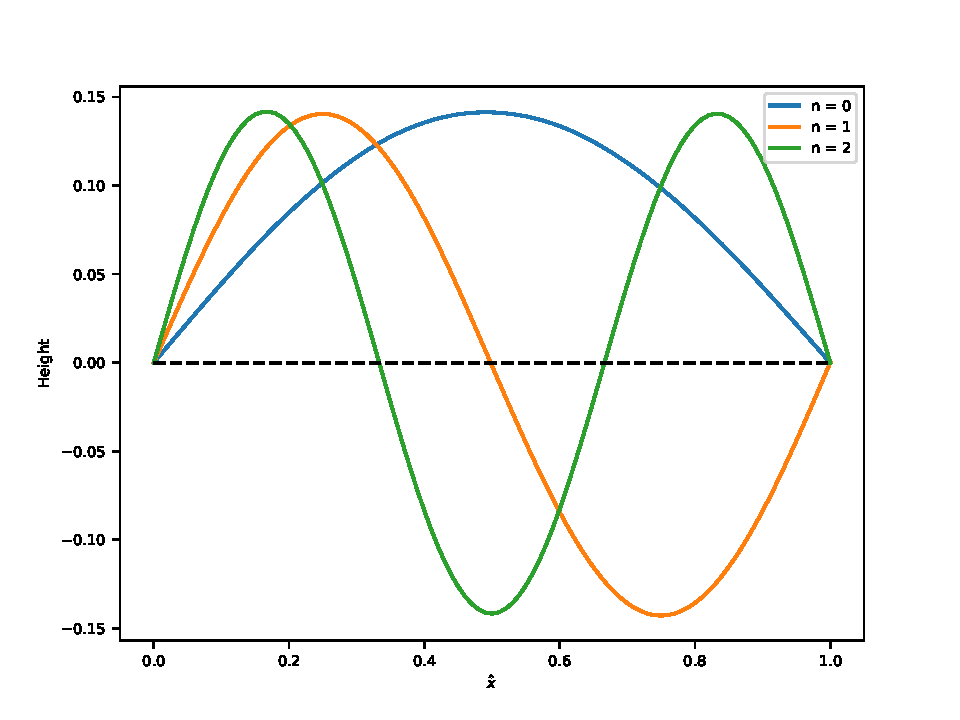
\includegraphics[width=1.0\linewidth]{figures/prob_6b.pdf}
				\caption{Numerical solution for the first three mode in plain line with the analytical solution for the same mode in red dashed line for N=100. The solution is presented with the dimensionless scale $\hat{x}$ is on the $x$-axis, and the amplitude is on the $y$-axis\label{fig:prob6b}}
			\end{figure}
		
		We have plotted in \autoref{fig:prob6b} the numerical and the analytical solution for the first three mode with different step size. We can see that in both case the numerical behavior is similar to what the theory predict. For this plot we have normalised the eigenvectors for the analytical solution with the \lstinline{arma::normalise} function introduce in the project description. We also had to multiply the second and third mode of the analytical solution by -1. This is not a problem because as we know if $v$ is a solution to our eigen system then $c*v$, with $c$ a constant, is also a solution.


\printbibliography[heading=bibintoc, title={References}]

\end{document}
